%!TEX program = xelatex
%!TEX encoding = UTF-8 Unicode

\documentclass[14pt, AutoFakeBold]{ldr}
  

\title{本 科 生 毕 业 答 辩}
\subtitle{Kubernetes存储插件性能测试对比及优化实践}

\author{答辩人:刘康恒}
\institute{指导老师:程刚}
\date{\today}
\titlegraphic{
\includegraphics[height=0.15\textwidth]{lzu_logo.png}}


\begin{document}

\maketitle

\AtBeginSection[]
{
  \begin{frame}
    \frametitle{目录}
    \tableofcontents[currentsection,hideallsubsections]
  \end{frame}
}

\section{研究背景}
\subsection{三级标题}

\begin{frame}
\frametitle{应用部署模式}
  企业应用部署模式回溯
\begin{itemize}
  \item 传统部署模式Bare Metal
  \item 虚拟化部署模式Virtual Machine
  \item 容器化部署模式Containerized Deployment
\end{itemize}
\end{frame}

\begin{frame}
  \frametitle{应用部署模式}
  \begin{figure}[H]
    \centering
    \includegraphics[width=1.0\textwidth]{deployments.png}
  
    \caption{部署模式演变}
    \label{deployments}
\end{figure}
\end{frame}

\begin{frame}
  \frametitle{Kubernetes容器管理平台}
  Kubernetes容器管理平台
  \begin{itemize}
    \item 2014年谷歌开源
    \item 2017年开放CSI驱动API
    \item 积极开发中 (每季度小版本推进)
  \end{itemize}
\end{frame}

\begin{frame}
  \frametitle{Ceph分布式存储}
  Ceph分布式存储
  \begin{itemize}
    \item 2006年开发
    \item 2017年开发CSI驱动适配Kubernetes集群
    \item 积极开发中 (每月份小版本推进)
  \end{itemize}
\end{frame}

\section{研究意义}
\begin{frame}
  \frametitle{研究意义}
  研究意义
  \begin{itemize}
    \item 开源
    \item 资源
  \end{itemize}
\end{frame}

\section{主要工作}
\begin{frame}
  \frametitle{主要工作}
  主要工作
  \begin{itemize}
    \item 搭建配置Kubernetes集群
    \item 搭建配置Ceph存储集群
    \item Kubernetes对接Ceph
    \item 后端存储性能测试
    \item 存储性能优化
  \end{itemize}
\end{frame}

\begin{frame}
  \frametitle{Kubernetes架构拓扑}
  \begin{figure}[H]
    \centering
    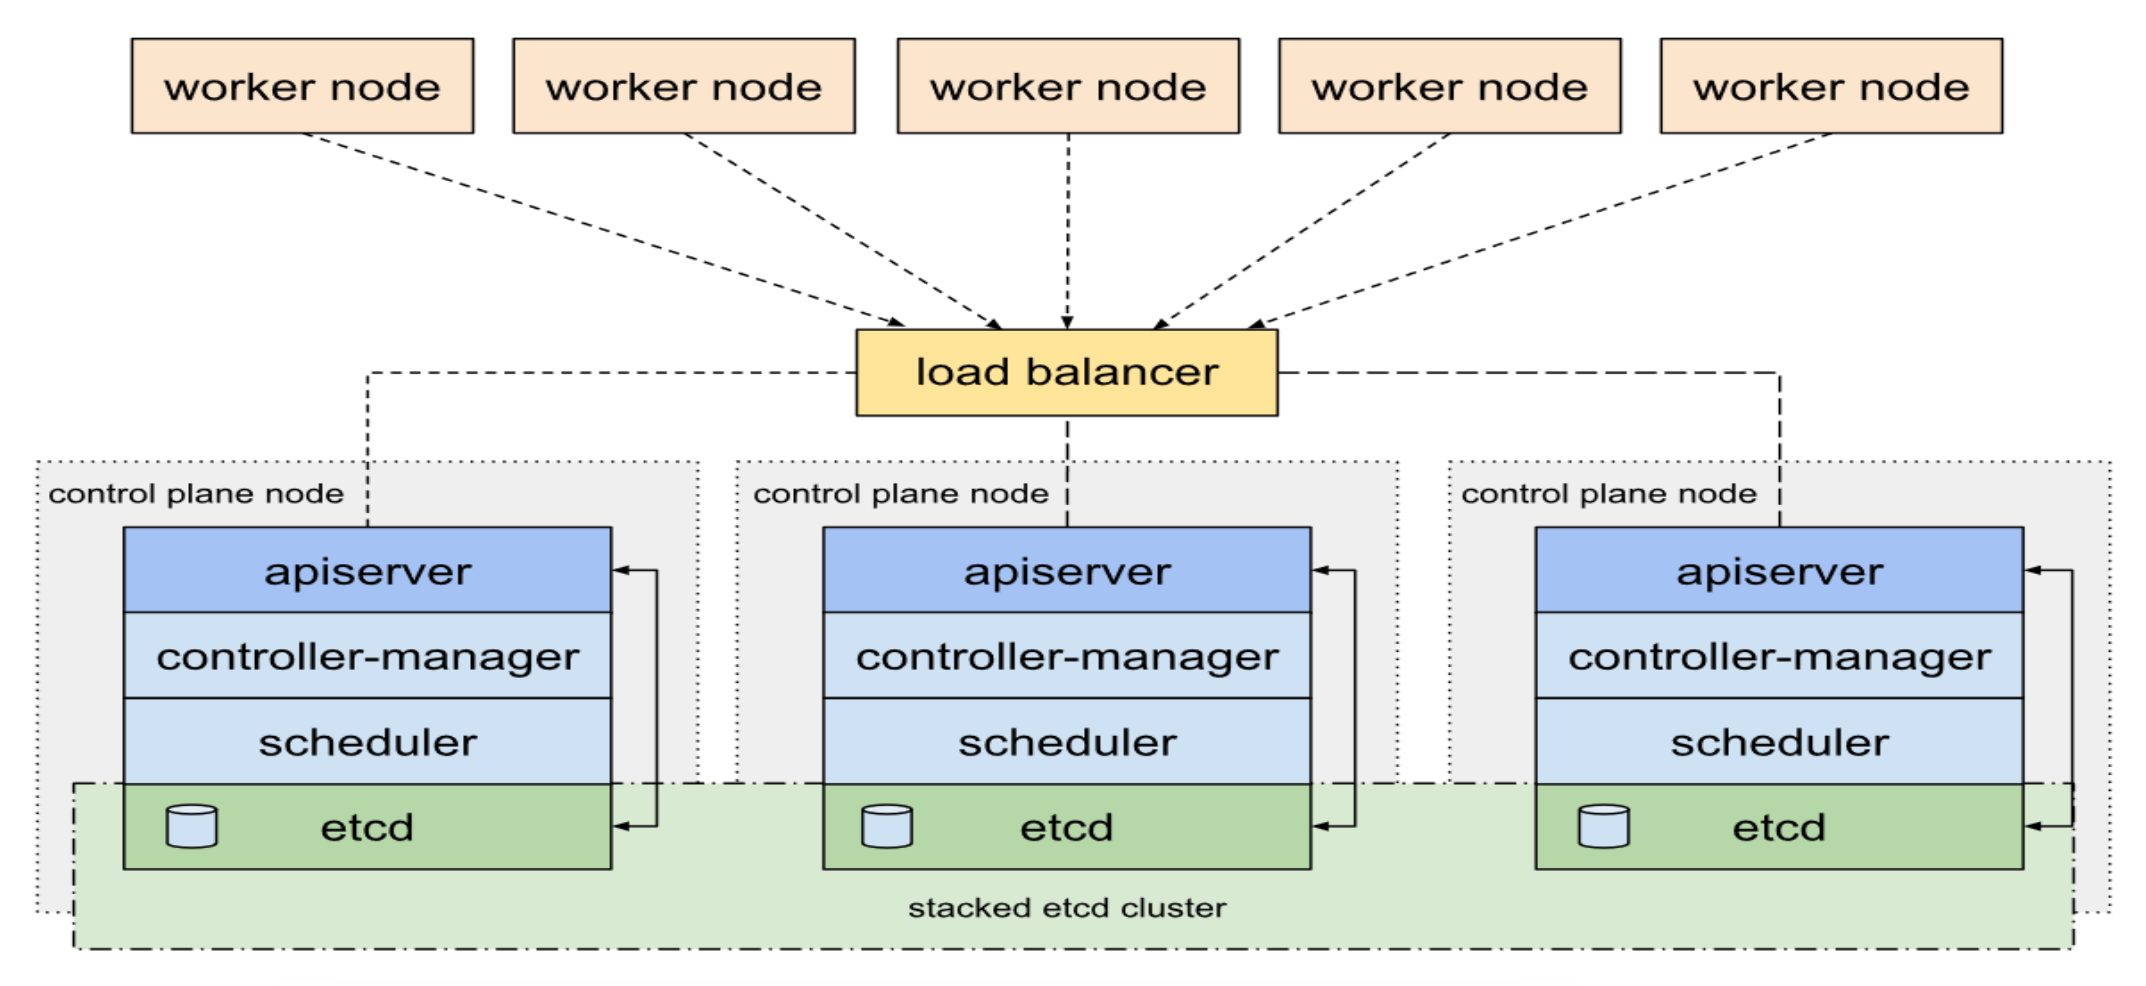
\includegraphics[width=1.0\textwidth]{kubetopology.png}
  
    \caption{Kubernetes架构拓扑}
    \label{kubetopology}
  \end{figure}
\end{frame}

\begin{frame}
  \frametitle{性能测试}
%   \begin{table}[H]
%     \centering
%     \caption{纳米管参数}
%     \begin{tabular}{cccccc} % 控制表格的格式
%         \toprule
%         参数 & m  & n  & 原子数 & 内径     & 长度    \\
%         \midrule
%         二硫化钼纳米管  & 15 & 15 & 3420   & 2.3014nm & 11.85nm \\
%         碳纳米管  & 16 & 6  & 1112   & 1.5424nm & 6.0nm   \\
%         \bottomrule
%     \end{tabular}
%     \label{tbl_mcnt_nanotube}
% \end{table}
\begin{table}[H] % 控制表格的格式,可以是l,c,r
  \caption{Sysbench文件I/O测试结果}
  \resizebox{\textwidth}{!}{
  \begin{tabular}{cccc}
    \toprule
  参数 & RBD & CephFS & NFS\\
    \midrule
  磁盘随机读写(MiB/s) & 21.56 读;14.38 写 & 22.32 读;14.88 写 & 6.28 读;4.19 写;\\
  磁盘顺序写入(MiB/s) & 123.20 & 147.17 & 99.25\\
  磁盘随机访问(MiB/s) & 5185.46 & 5790.62 & 5684.66\\
  % 数值3 & 15 & 15 & 15\\
    \bottomrule
  \end{tabular}
  }
\end{table}
\end{frame}
% \begin{frame}[c]{列表怎么用}
% 就是下面这么用,前面是个点点,原因是我在模板里自定义了,你可以修改,模板中搜索:列表前面的点点自定义
%   \begin{itemize}
%   \item 简捷易行
%   \item 保存原文的格调和“洋味”
%   \item[1] 你是可以用数字的
%   \item[2] 你是可以用数字的
%   \end{itemize}
% 还有这一种,也挺好看的
%   \begin{enumerate}
%     \item 测试
%     \item 测试
%   \end{enumerate}
% \end{frame}




% \begin{frame}
%   \frametitle{每一页内容位置}

%   内容老是居中,我想让它居上怎么办?看下一页


% \end{frame}

% \begin{frame}[t]{每一页内容位置}

%   这句话在上面了吧,原因是上面那个[t],默认[c](居中)


% \end{frame}



% \section{主要内容}

% \begin{frame}
%   \frametitle{图并排}
%   \begin{figure}[H]
%     \centering
%     
\includegraphics[width=0.3\textwidth]{lzu_logo.png}
  
%     \caption{兰州大学(单图)\footnotesize 小字可以这么来}
%     \label{fig_lzu}
% \end{figure}
  
% \end{frame}
% \begin{frame}
%   \frametitle{图并排}
%   \begin{figure}[H]
%     \centering
%     \subfloat[图1]{
%         \label{fig_lzus_0}
%         
\includegraphics[width=0.3\textwidth]{lzu_logo.png}
%     }
%     \subfloat[图2]{
%         \label{fig_lzus_1}
%         
\includegraphics[width=0.3\textwidth]{lzu_logo.png}
%     }\\
%     \caption{兰州大学}
%     \label{fig_lzus}
% \end{figure}
  
% \end{frame}


% \begin{frame}
%   \frametitle{表格}
%   \begin{table}[H]
%     \centering
%     \caption{纳米管参数}
%     \begin{tabular}{cccccc} % 控制表格的格式
%         \toprule
%         参数 & m  & n  & 原子数 & 内径     & 长度    \\
%         \midrule
%         二硫化钼纳米管  & 15 & 15 & 3420   & 2.3014nm & 11.85nm \\
%         碳纳米管  & 16 & 6  & 1112   & 1.5424nm & 6.0nm   \\
%         \bottomrule
%     \end{tabular}
%     \label{tbl_mcnt_nanotube}
% \end{table}
% \end{frame}

% \begin{frame}
% \frametitle{左右分栏}
% 去掉 pause  就不会变成两页了
%   \begin{columns}
%   \column{0.6\textwidth}

%     \begin{itemize}
%     \item Ice Age
%     \item The Hobbit
%     \item The Great Gatsby
%     \end{itemize}
%   \pause
%   \column{0.4\textwidth}
%     \begin{itemize}
%     \item 冰河世纪
%     \item 霍比特人
%     \item 了不起的盖茨比
%     \end{itemize}
%   \end{columns}
% \end{frame}

% \begin{frame}
%   \frametitle{分步动画}


%   \onslide<1>{
%     第一步显示这一句话,第二步时消失在
%   }
%   \onslide<2,3>{
%     \begin{block}{解析:}
%       第二、三步显示这一句话
%     \end{block}
%   }

%   \onslide<3>{
%     只有第三步显示这一句话
%   }

% \end{frame}

\section{展望}
\begin{frame}
  \frametitle{展望}
  展望
  \begin{itemize}
    \item 扩展至其他后端存储
    \item 模拟仿真
  \end{itemize}
\end{frame}
% \begin{frame}
%   \frametitle{测试}

%   \begin{block}{方框}
%     测试一下,参考一篇文献\cite{partl2016}
%   \end{block}

% \end{frame}


% \section{参考文献}
% \begin{frame}[t]
%   \frametitle{参考文献}
%   % 这里会把ppt引用的参考文献全部在这里显示
%   \bibliographystyle{bib/lzubib}
%   \bibliography{bib/database}
  
% \end{frame}

\section{致谢}

% \begin{frame}[t]
% \frametitle{致谢}
%   % 注意致谢内容答辩时不要读出来,播放到这里就可以了
%   \begin{itemize}
%   \item 感谢老师
%   \item 感谢同学
%   \item 感谢学校
%   \item 感谢父母
%   \item 也可以感谢我 ~
%   \end{itemize}
% \end{frame}






\end{document}